\chapter{宏}\label{ch21}

\emph{A cento (from the Latin for “patchwork”) is a poem made up entirely of lines quoted from another poet.}
\begin{flushright}
    ——Matt Madden
\end{flushright}

Rust支持\emph{宏(macros)}:一种普通函数无法做到的扩展语言的方式。例如,我们已经看到过\texttt{assert\_eq!}宏,它可以方便地用来测试:
\begin{minted}{Rust}
    assert_eq!(gcd(6, 10), 2);
\end{minted}

这也可以写成一个泛型函数,但\texttt{assert\_eq!}可以做到几件函数做不到的事。一是当断言失败时,\texttt{assert\_eq!}会生成包含断言所在的文件名和行号的错误消息。函数没有办法获得这些信息。但宏可以,因为它们工作的方式完全不同。

宏是一种缩写。在编译期间,在类型检查之前、更在生成任何机器码之前,每一个宏调用都会被\emph{展开(expand)}——即,被替换为一些Rust代码。上面的宏调用会展开成类似这样的代码:
\begin{minted}{Rust}
    match (&gcd(6, 10), &2) {
        (left_val, right_val) => {
            if !(*left_val == *right_val) {
                panic!("assertion failed: `(left == right)`, \
                        (left: `{:?}`, right: `{:?}`)", left_val, right_val));
            }
        }
    }
\end{minted}

\texttt{panic!}也是一个宏,它自己会展开成更多Rust代码(这里没有展示)。那些代码里用到了两个别的宏,\texttt{file!()}和\texttt{line!()}。一旦crate中的每一个宏调用都被完全展开,Rust会进入编译的下一个阶段。

在运行时,一个断言失败看起来像这样(并且可能指示\texttt{gcd()}函数中的一个bug,因为\texttt{2}是正确的答案):
\begin{minted}{text}
    thread 'main' panicked at 'assertion failed: `(left == right)`, (left: `17`,
    right: `2`)', gcd.rs:7
\end{minted}

如果你是从C++来的,你可能经历过一些宏的糟糕体验。Rust的宏采用了一种不同的方式,类似于Scheme的\texttt{syntax-rules}。相比于C++的宏,Rust的宏和语言的其他部分集成得更好,并且因此更不容易出错。宏调用总是用感叹号标记,这样当你阅读代码时它们会很显眼,并且不会在你想调用函数时偶然错误地调用成了宏。Rust的宏从来不会插入不匹配的花括号或圆括号。并且Rust的宏带有模式匹配,这使得编写既可维护又易于使用的宏变得更容易。

在本章中,我们将通过几个简单的示例展示如何编写宏。但和Rust中的很多部分一样,宏值得深入理解,所以我们将介绍一个更复杂的宏的设计,它允许我们直接在我们的程序中嵌入JSON字面量。但除了本书中介绍的部分之外,宏还有更多的内容。因此我们将以一些进一步学习的点结束,既有我们将在这里向你展示的高级技巧,也有功能更加强大的设施称为\emph{过程宏(procedural macros)}。

\section{宏基础}
\autoref{f21-1}展示了\texttt{assert\_eq!}宏的部分源码。

\begin{figure}[htbp]
    \centering
    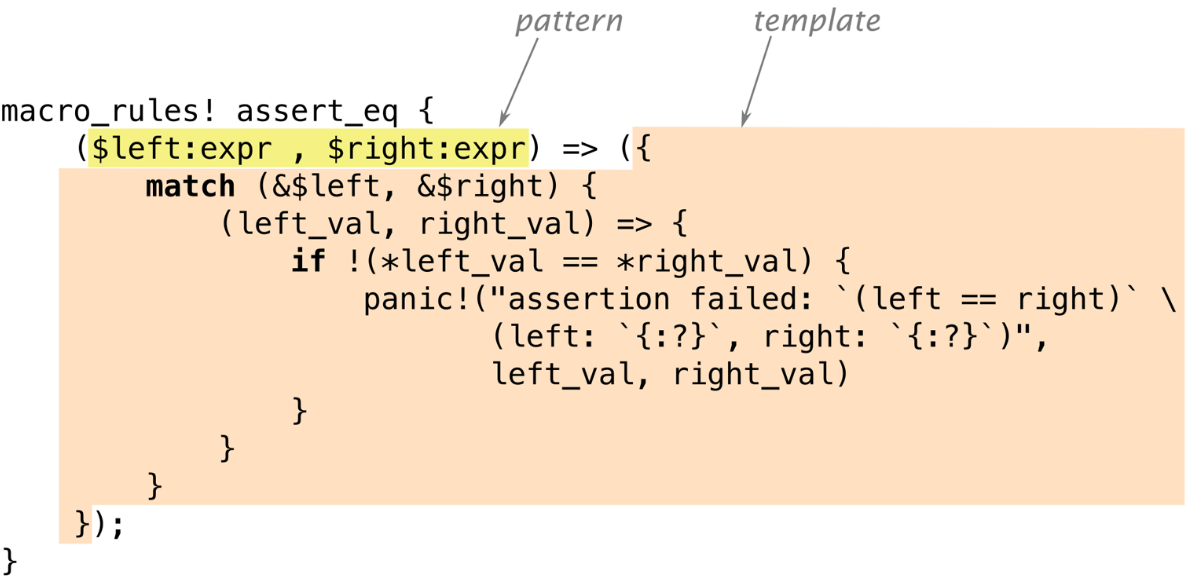
\includegraphics[]{../img/f21-1.png}
    \caption{\texttt{assert\_eq!}宏}
    \label{f21-1}
\end{figure}

\texttt{macro\_rules!}是Rust中定义宏的主要方法。注意,宏定义里\texttt{assert\_eq}后边没有\texttt{!}:只有在调用宏时才需要\texttt{!},定义时不需要。

并不是所有的宏都是以这种方式定义的:少数的宏,例如\texttt{file!}、\texttt{line!}和\texttt{macro\_rules!}自身,是编译器内建的。我们将在本章的末尾讨论另一种方法,称为过程宏。但我们的主要精力还是集中在\texttt{macro\_rules!},这是(目前为止)最容易的编写自己的宏的方法。

一个用\texttt{macro\_rules!}定义的宏完全靠模式匹配工作。宏的主体只是一系列规则:
\begin{minted}{text}
    ( pattern1 ) => ( template1 );
    ( pattern2 ) => ( template2 );
    ...
\end{minted}

\autoref{f21-1}中的\texttt{assert\_eq!}版本只有一个模式和一个模板。

顺便,你可以使用方括号或者花括号来代替模式或模板两侧的圆括号,对Rust来说它们并没有任何区别。另外,当你调用一个宏时,这些都是等价的:
\begin{minted}{Rust}
    assert_eq!(gcd(6, 10), 2);
    assert_eq![gcd(6, 10), 2];
    assert_eq!{gcd(6, 10), 2}
\end{minted}

唯一的不同是花括号后边的分号是可选的。为了方便,我们在调用\texttt{assert\_eq!}时使用圆括号,调用\texttt{vec!}时使用方括号,\texttt{macro\_rules!}时使用花括号。

现在我们展示了一个宏展开的简单示例和生成这个宏的定义,我们可以深入了解它工作的细节:
\begin{itemize}
    \item 我们将详细地解释Rust是怎么发现和展开你的程序中的宏定义的。
    \item 我们将指出在根据宏模板生成代码时的一些细节之处。
    \item 最后,我们将展示模式如何处理重复的结构。
\end{itemize}

\subsection{宏展开基础}
Rust会在编译的前期展开宏。编译器会从头到尾读取源码,在这个过程中定义和展开宏。宏只有在定义之后才能被调用,因为Rust会立刻展开每一个宏调用,而不会去看程序的剩余部分。(相反,函数和其他的\hyperref[static]{item}的定义不需要按照任何顺序。调用一个后面才定义的函数也是OK的。

当Rust展开一个\texttt{assert\_eq!}宏调用时,行为和执行一个\texttt{match}表达式非常像。Rust首先根据模式匹配参数,如\autoref{f21-2}所示:
\begin{figure}[htbp]
    \centering
    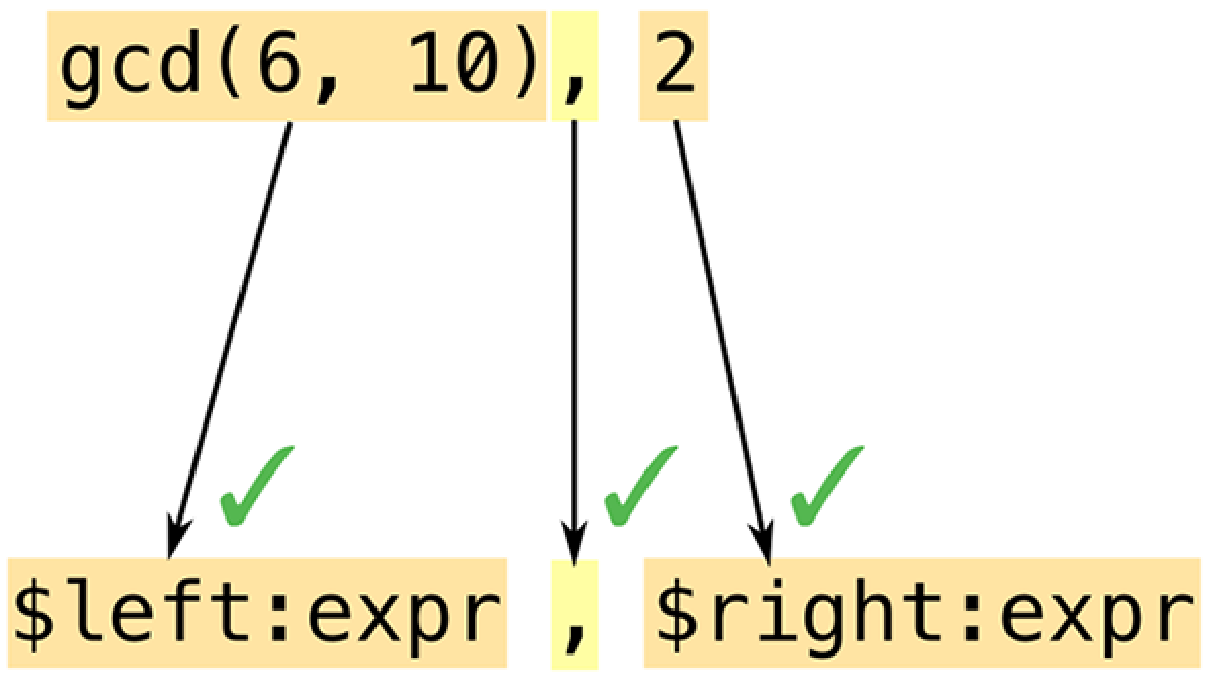
\includegraphics[width=0.8\textwidth]{../img/f21-2.png}
    \caption{展开一个宏,第1部分:用模式匹配参数}
    \label{f21-2}
\end{figure}

宏的模式是Rust的mini语言。它们本质上是匹配代码的正则表达式。但普通的正则表达式是操作字符,而模式操作\emph{token(词元)}——数字、变量名、标点符号等Rust中的构建块。这意味着你可以在宏模式中自由地使用注释和空格来提升它们的可读性。注释和空格不是token,因此它们不会影响到匹配。

正则表达式和宏模式的另一个重要不同之处是圆括号、方括号、花括号在Rust中总是成对出现。这一点会在宏展开之前就检查,不仅仅是在宏模式中,而且是在整个语言中。

在这个例子中,我们的模式包含了\emph{fragment(片段)} \texttt{\$left:expr},这告诉Rust去匹配一个表达式(在这个例子中,就是\texttt{gcd(6, 10)}并把它复制到名称\texttt{\$left}。然后Rust用\texttt{gcd}调用后边的逗号匹配模式中的逗号。类似于正则表达式,模式只有少数特殊字符会触发有趣的匹配行为;其它的所有字符,例如逗号,都必须逐字匹配相同的字符,否则就会匹配失败。

这个模式中的两个代码片段都是\texttt{expr}类型:它们代表表达式。我们将在“\nameref{FragType}”中看到其他类型的代码片段。

因为这个模式匹配到了所有的参数,Rust会展开相应的\emph{template(模板)}(\autoref{f21-3}):
\begin{figure}[htbp]
    \centering
    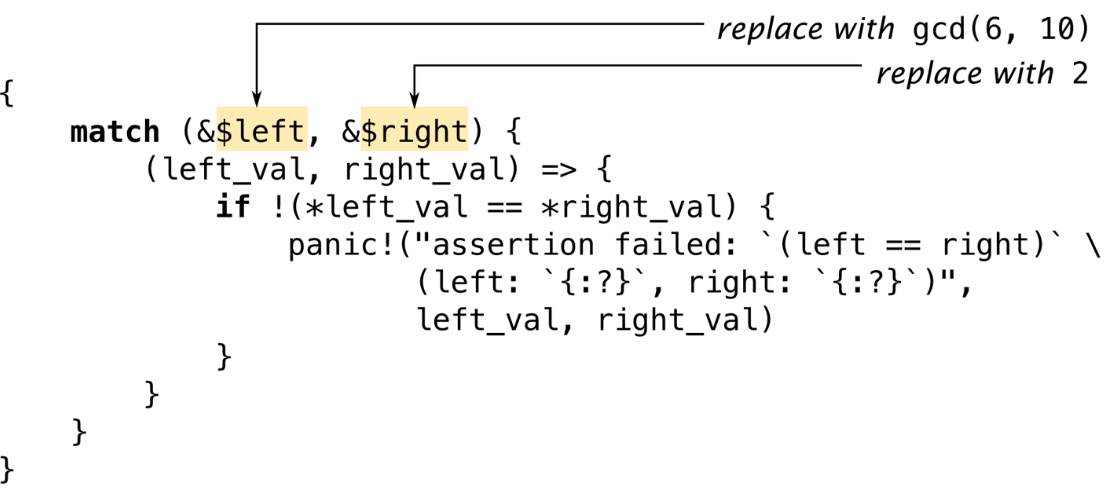
\includegraphics[width=0.9\textwidth]{../img/f21-3.png}
    \caption{展开一个宏,第2部分:填充模板}
    \label{f21-3}
\end{figure}

Rust会用匹配阶段发现的代码片段来替换\texttt{\$left}和\texttt{\$right}。

一个常见的错误是在输出模板中包含片段的类型:写\texttt{\$left:expr}而不是\texttt{\$left}。Rust不会立刻检测出这种错误。它会把\texttt{\$left}看错一个整体,然后把\texttt{:expr}看作和模板中其他部分一样的东西:要包含在宏的输出中的词元。因此只有当你\emph{调用}这个宏时这个错误才会出现;然后它会生成错误的不能编译的输出。如果你在使用一个新的宏时得到了类似\texttt{cannot find type `expr` in this scope}和\texttt{help: maybe you meant to use a path separator here}这样的错误消息,可以检查下它是不是有这个错误。(“\nameref{DebugMacro}”提供了更多类似这种情况的建议。)

宏模板和web编程中常用的很多种模板语言中的任意一种都没有太大的区别。唯一的不同——也是很重要的一点——就是它的输出是Rust代码。

\subsection{意外后果}

\section{内建的宏}


\section{调试宏}\label{DebugMacro}


\section{构建\texttt{json!}宏}


\subsection{片段类型}\label{FragType}
